\documentclass[./exercises.tex]{subfiles}

\begin{document}
\noindent\textbf{Tentamen 2021-06-02 fråga 5}\hfill\break
Temperaturen i ett kylskåp ska vara $0.0^\text{o}$C,
och rummet i vilket kylskåpet är placerat
har temperaturen $+20^\text{o}$C.
Hur stor effekt måste vi tillföra kylmaskinen,
om denna är en ideal carnotmaskin
och det per dygn läcker in $10^7$ J värme i kylskåpet.

\begin{table}[ht]
\noindent\begin{tabular}{ l l l  } 
Givet&  				   & Sökt\\
$T_1$&= $293^\text{o}$K & $\dot{W}$\\
$T_2$&= $273^\text{o}$K    &\\ 
$\dot{Q}$&= $10^7$ J/dygn  &\\       
\end{tabular}
\end{table}



\begin{figure}[h]
\centering
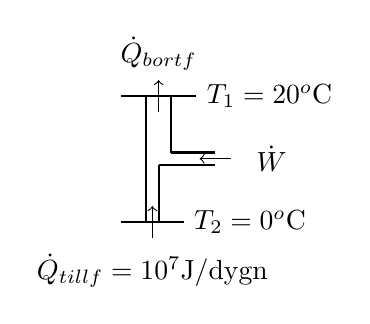
\begin{tikzpicture}[ scale=.4,baseline={(0,0)}]
%\draw upper 

\draw [thick] (1,0) -- (3,0) node[right]{    $T_2=0^o$C};%Basen för Q tillförd

\draw [thick] (1,4) -- (3.4,4) node[right]{    $T_1=20^o$C};%Basen för Q bortförd
\draw [thick] (1.8,0) -- (1.8,4); %Vänster kanalvägg
\draw [thick] (2.2,0) -- (2.2,1.8); %Höger kanalvägg
\draw [thick] (2.2,1.8)--(4,1.8); %w nedre kanalvägg
\draw [thick] (4,2.2)-- (2.6,2.2); %w övre kanalvägg
\draw [thick] (2.6,2.2)-- (2.6,4); %höger kanalvägg upp till bas

\draw[->] (2,-0.5) -- (2,0.5);
\node[below] (a) at (2,-0.7){$\dot{Q}_{tillf}=10^7$J/dygn};

\draw[->] (4.5,2) -- (3.5,2);
\node[right] (b) at (5,2){$\dot{W}$};

\draw[->](2.2,3.5)--(2.2,4.5) node[above]{$\dot{Q}_{bortf}$};

\end{tikzpicture}
\end{figure}

$\dot{Q}_{tillf}=107$J/dygn, vilket blir $10^7/(24\cdot 3600)$W.
Carnotmaskinen arbetar såsom kylmaskin.
Vi vet att den teoretiska verkningsgraden $\eta_c$ för Carnotmaskin såsom värmemotor härletts
från uttrycket för den den teoretiska verkningsgraden $eta_t$ i det allmänna fallet
\begin{flalign*}
\eta_t &=\frac{q_{tillf}-|q_{bortf}|}{q_{tillf}} &\\
       &=\frac{w}{q_{tillf}} &(1)\\
\eta_c &= 1-\frac{T_1}{T_2} &\\
       &=\frac{T_2-T_1}{T_2}&(2)\\
\end{flalign*}
och i boken väljer man $T_1$ som den lägre temperaturen när man avhandlar värmemotorer
men konventionen i boken är tvärtom för kylmaskiner för då definierar man $T_1$ som den högre temperaturen
och därför har vi valt variabelbeteckningarna som vi har gjort. 
Men vi har nu en kylmaskin och för en sådan definieras den s.k. köldfaktorn
istället för verkningsgraden.
\begin{flalign*}
\epsilon_t &=\frac{q_{tillf}} {|q_{bortf}|-q_{tillf}}&(3)\\
       &=\frac{q_{tillf}}{w} &(4)\\
\end{flalign*}
Observera att för värmemotorn gäller
\begin{flalign*}
w &=q_{tillf} - |q_{bortf}| &(5)\\
\end{flalign*}
men för kylmaskinen gäller
\begin{flalign*}
w &=  |q_{bortf}|-q_{tillf}&(6)\\
\end{flalign*}
Från det utritade kanalernas bredder så ser man att ekvation (6)
stämmer med vad som ritats ut
\begin{flalign*}
w +q_{tillf}&=  |q_{bortf}|&\\
\end{flalign*}
På samma sätt så måste man för att rita korrekt schematisk figur för en värmemotor så måste det då
ur ritningen framgå ur de utritade bredderna på kanalerna att
\begin{flalign*}
w +|q_{bortf}| &=q_{tillf} &\\
\end{flalign*}

Vi vill beräkna carnotködfaktorn och sätta det värdet lika med ekvation (3)
men formeln finns inte i formelsamlingen så vi måste göra härledningen
enligt boken på sidan 317.
För en Carnot kylmaskin har vi följande $T\mhyphen s$ diagram

\begin{figure}[h]
\centering
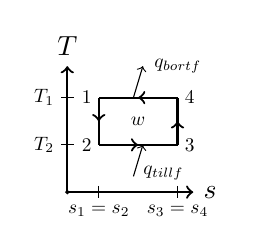
\begin{tikzpicture}[scale=.4,baseline={(0,0)}]
%\begin{tikzpicture}[show background rectangle, scale=.5]

%\draw (0,0) grid (4,4);
% x-axis
\draw [thick,->] (0,0) -- (4,0) node[right]{$s$};
% y-axis
\draw [thick,->] (0,0) -- (0,4) node[above]{$T$};
% x-axis label
%\node at (-0.3,4){$T$};
% y-axis label
%\node at (4,-0.3){$s$};
%origin point
\draw [color=black,fill=black] (0,0) circle (0.05);

\draw[thick](1,1.5)--(3.5,1.5)node[scale=0.7, right]{3};
\draw[thick,->](1,1.5)--(2.25,1.5);

\draw[thick](3.5,1.5)--(3.5,3)node[scale=0.7,right]{4};
\draw[thick,->](3.5,1.5)--(3.5,2.25);

\draw[thick](3.5,3)--(1,3)node[scale=0.7, left]{1};
\draw[thick,->](3.5,3)--(2.25,3);

\draw[thick](1,3)--(1,1.5)node[scale=0.7, left]{2};
\draw[thick,->](1,3)--(1,2.25);

\draw[->](2.1,0.5)--(2.4,1.5);%q_tillf pil
\draw[->](2.1,3)--(2.4,4);%q_bortf pil

\node[right,scale=0.7] (a) at (2.2,0.6){$q_{tillf}$};
\node[scale=0.7] (c) at (2.25,2.25){$w$};
\node[right,scale=0.7] (d) at (2.55,4.0){$q_{bortf}$};

\draw (1,0.2)--(1,-0.2) node[below,scale=0.7]{$s_1=s_2$};
\draw (3.5,0.2)--(3.5,-0.2) node[below,scale=0.7]{$s_3=s_4$};

\draw(0.2,3)--(-0.2,3) node[left,scale=0.7]{$T_1$};
\draw(0.2,1.5)--(-0.2,1.5) node[left,scale=0.7]{$T_2$};

\end{tikzpicture}
\end{figure}

Vi ska nu teckna $\epsilon_c$
\begin{flalign*}
\epsilon_c &=\frac{q_{tillf}} {|q_{bortf}|-q_{tillf}}&\\
       &=\frac{T_2\cdot (s_3-s_1)} {T_1\cdot(s_3-s_1)-T_2\cdot (s_3-s_1)}&\\
       &=\frac{T_2} {T_1-T_2}&(7)\\
\end{flalign*}
Vilket för vårat fall blir
\begin{flalign*}
\epsilon_c &=\frac{273} {293-273}&(8)\\
\end{flalign*}
Kvoten mellan flödena av $q_{tillf}$ och $w$ måste ge samma kvot utan tidsderivering
\begin{flalign*}
\epsilon_t &=\frac{\dot{q}_{tillf}}{\dot{w}}&(9)\\
           &=\frac{\dot{Q}_{tillf}}{\dot{W}}&(10)\\
\end{flalign*}
Vi sätter nu $(10)$ och $(8)$ lika med varandra
\begin{flalign*}
\frac{T_2} {T_1-T_2}&=\frac{\dot{Q}_{tillf}}{\dot{W}}&\\
\dot{W} &=\frac{\dot{Q}_{tillf}\cdot (T_1-T_2)}{T_2}&\\
        &=\frac{10^7}{24\cdot 3600}\cdot \frac{293-273}{273}&\\
        &= 8.479175146 \text{W}
\end{flalign*}



Detta ska avrundas till två värdesiffror eftersom minsta antalet
värdesiffror i problemformuleringen ges av 0.0 so har två värdesiffror
och 20 som antingen har två eller 1 värdesiffra.
0.0 har två värdesiffror i enligt regeln
\textit{``nollan i slutet räknas eftersom den kommer efter
ett decimalkomma och det finns andra värdesiffror före decimalkommat"}
\footnote{\url{https://web.archive.org/web/20220514213530/https://grundskoleboken.se/wiki/Avrundning}}
Således måste vi tillföra effekten 8.5 W.

\end{document}